In order to qualify as an author in the ATLAS collaboration a task must be completed as a contribution to the experiment. The assigned task was to study the  impact of service material from the recent Insertable B-Layer (IBL) upgrade on the transverse momentum reconstruction in the forward region. Throughout this task, a large portion of the software required for the thesis analysis was developed because this specific qualification work was chosen with the currently proposed analysis in mind. 

The IBL was installed during LS1 between 2013 and 2015. This new pixel detector was needed to achieve better vertex resolution during the higher luminosity Run 2. The service materials, which run out azimuthally from the beam-pipe in high pseudorapidity regions were found to have very high radiation lengths compared to the material previously there. This could have a negative impact on the forward calorimeter's performance.

In order to better understand the effect of the IBL services on forward physics, specifically forward jet measurements, the azimuthal dependence of $\Delta\phi$, and relative $p_{T}$ response in a forward-central dijet system, as well as azimuthal jet yields were looked at in 5.02~TeV $pp$ data and MC samples. Additionally, jet response and $\Delta\phi$ correlations between truth and reconstructed jets in MC were also studied.

\section{Event Selection and Cuts}
Data from the heavy ion 5.02~TeV $pp$ run in 2015 was used and selected by forward High Level Triggers.
The Monte-Carlo samples used were generated by PYTHIA~8 \cite{Sjostrand:2014zea}, with leading order PDFs, and simulated by GEANT4 \cite{Agostinelli:2002hh, Aad:2010ah}.

The relative azimuthal angular correlation, $\Delta\phi$, between forward and central, leading and sub-leading jets, was studied at as a function of the central jets' azimuthal angle $\phi$. A 20 GeV $p_{T}$ cut was placed on the central jet, and different cuts were placed on the forward jets. Three jet events were rejected if $40\%$ of the average $p_{T}$ of the two leading jets was less than the $p_{T}$ of the third jet. Initially, jets were required to be isolated such that if two jets fall within a cone of $R=1.0$, then one jet has to have at least twice the transverse momentum of the second jet. 

\section{Procedure}
Throughout this study, using the specified data and MC samples, jets were reconstructed using the anti-$k_{T}$ algorithm with a radius of $R=0.4$ \cite{Cacciari:2008qp}. Topological towers with a $\Delta\eta\times\Delta\phi = 0.1\times0.1$ were constructed from calorimeter information and used as input into the clustering jet reconstruction algorithm. The HI jet calibration was used along with standard event selection cuts. This is the same calibration used in the main thesis analysis and will be discussed in more detail in Chapter~\ref{sec:mainanalysis}.

Azimuthal jet yields in bins of pseudorapidity, azimuth, and transverse momentum were normalized to the mean in each bin to get the normalized azimuthal jet yield.

\begin{equation}
Normalized\ Yield(p_{T},\eta,\phi) = \frac{Yield(p_{T},\eta,\phi) - Mean\ Yield(p_{T},\eta)}{Mean\ Yield(p_{T},\eta)}
\end{equation}

Both the $\Delta\phi$ and relative $p_{T}$ distributions were filled in bins of $\eta$, $p_{T}^{Forward}$, and $\phi_{Central}$. For every $\phi_{Central}$ bin, the respective distribution was fitted to a Gaussian, as shown in Figure~\ref{fig:fitting}, with some $\Delta\phi$ fits as an example, to yield the final azimuthal distributions.

\begin{figure}
	\centering
	{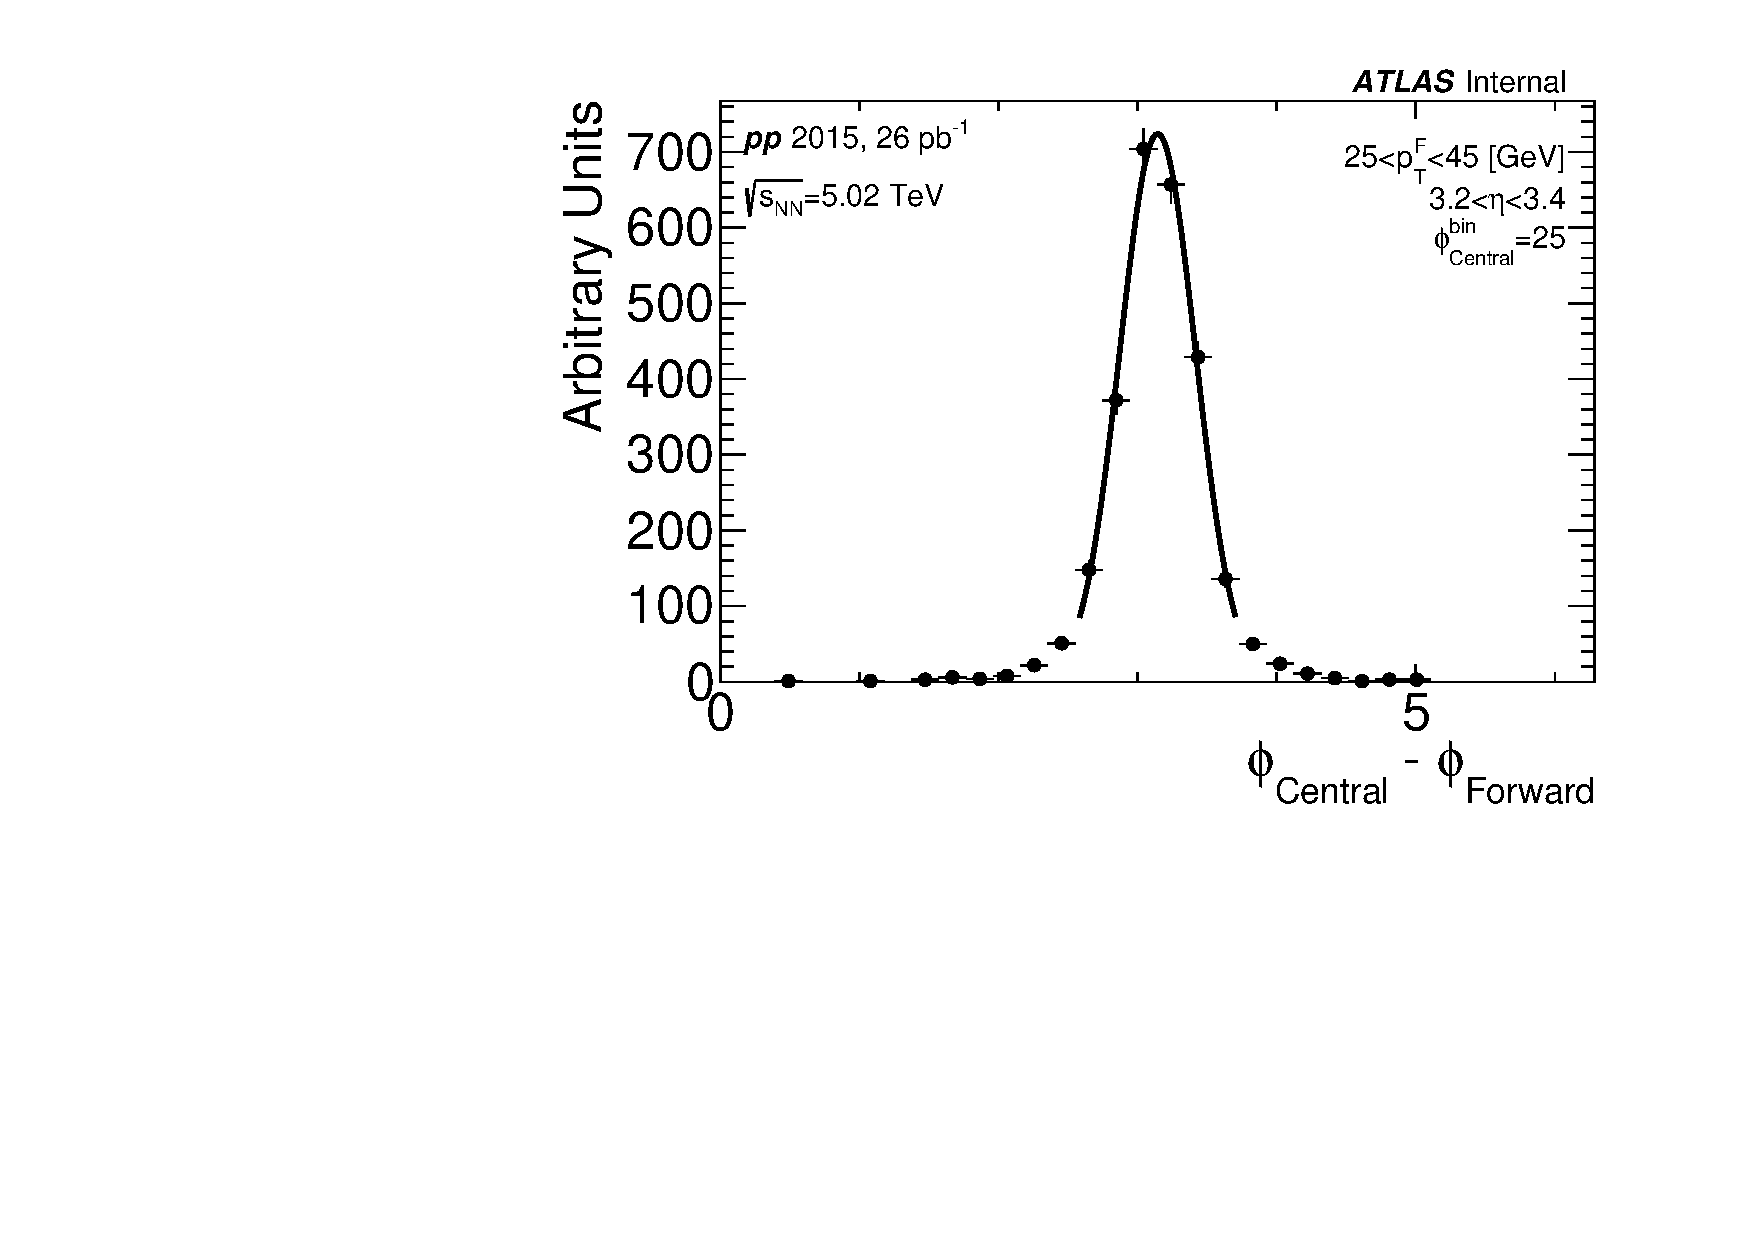
\includegraphics[width=0.45\textwidth]{figures/qualification/dPhiFit1.pdf}}
	{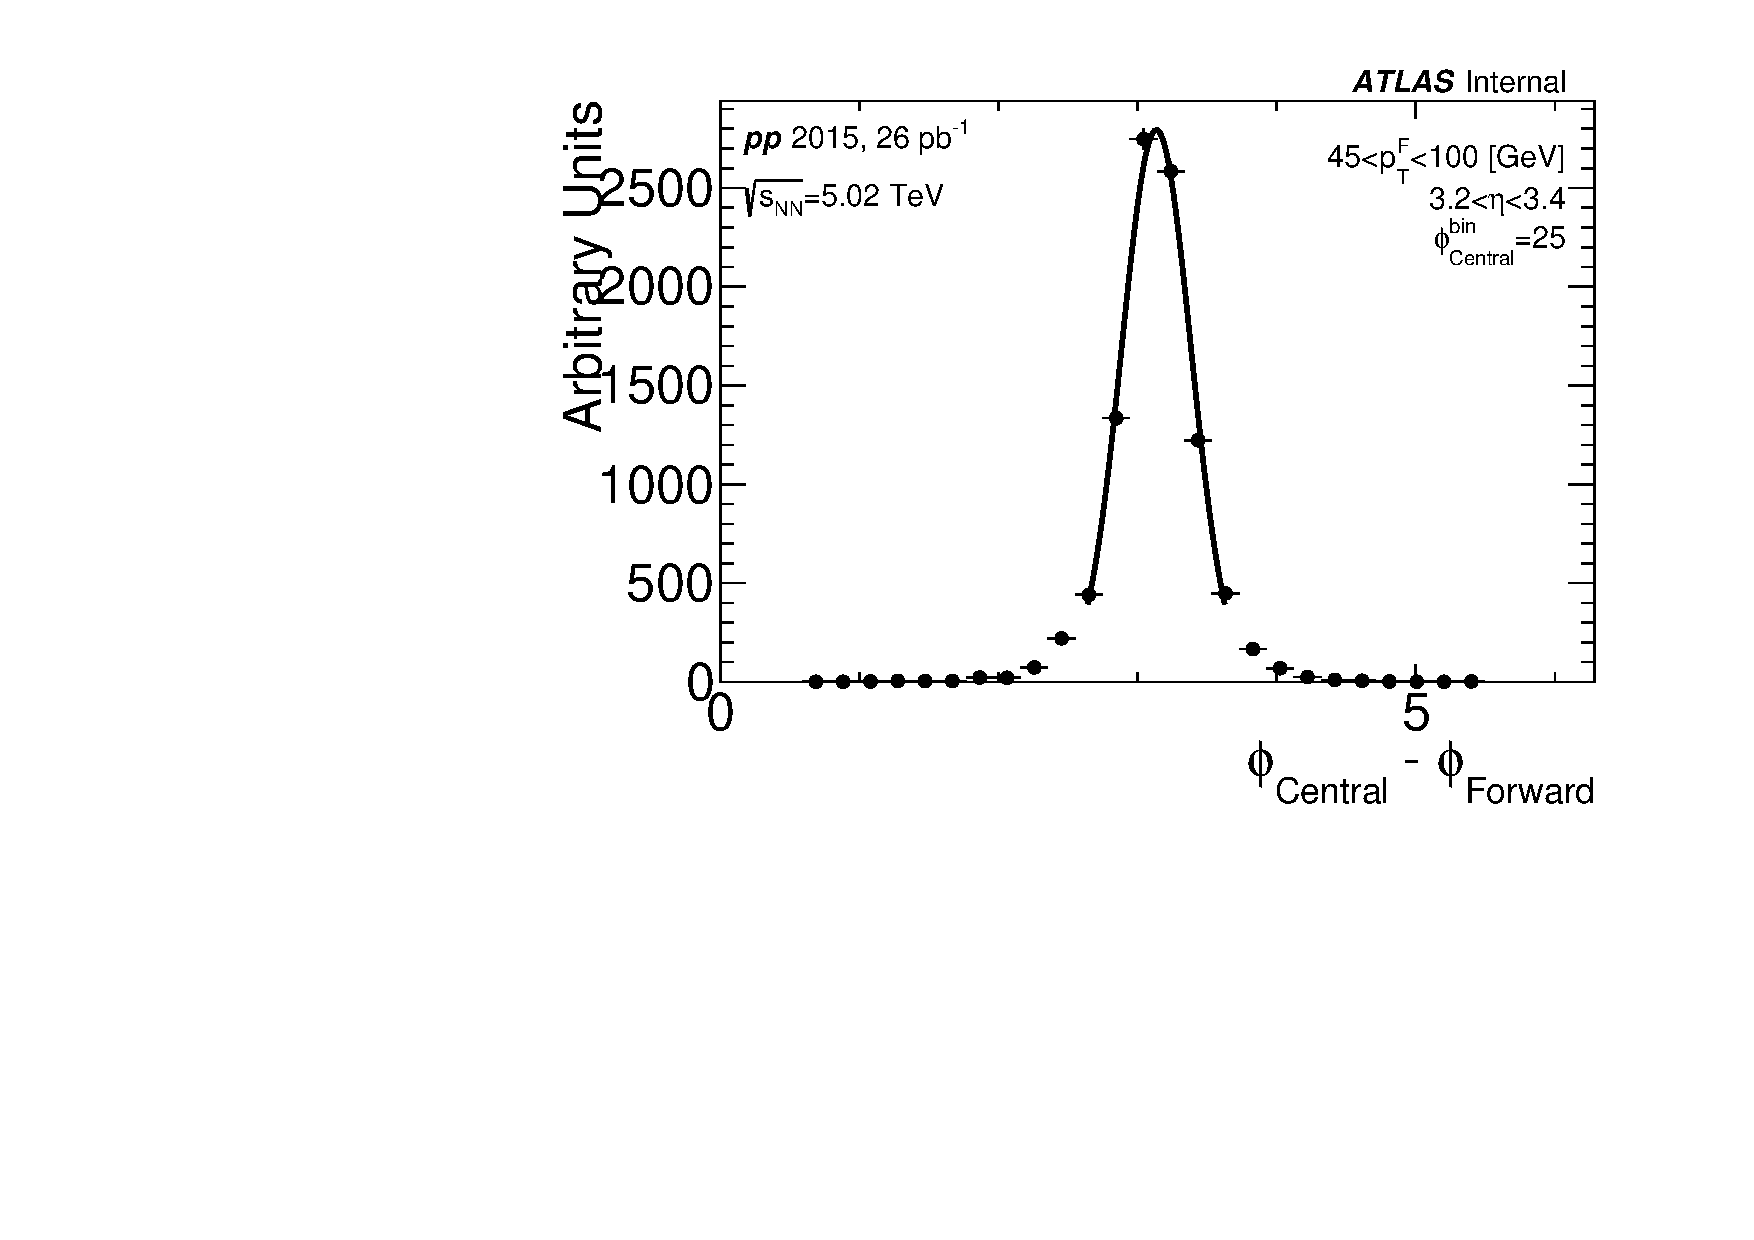
\includegraphics[width=0.45\textwidth]{figures/qualification/dPhiFit2.pdf}} %
	\caption{Examples of Gaussian fitted $\Delta\phi$ distributions in various $\eta$, $p_{T}^{Forward}$, and $\phi_{Central}$ bins.}%
	\label{fig:fitting}%
\end{figure}

\section{Results}

For both IBL and non-IBL regions, one forward $p_{T}$ bin is selected and the normalized yield distributions are plotted for both data and MC in Figure~\ref{fig:mcdata}. The magnitude of the variation in the IBL and non-IBL regions is similar in the data, while in MC it is flat in the non-IBL region, but oscillates in the IBL region. In the data, however, there is even some modulation in the non-IBL region. 

Looking at the RMS of the projections onto the y-axis, in the non-IBL region ($3.6<\eta<3.8$) the data has an $RMS=0.20$ while the MC has an $RMS=0.098$, and the IBL region ($3.8<\eta<4.4$) the data has an $RMS=0.21$ and the MC an $RMS=0.16$. This shows that in the data, the two regions are not so different, but they are in the MC. This is due to the IBL services being described differently in the MC than what is actually seen in the data. 

\begin{figure}
	\centering
	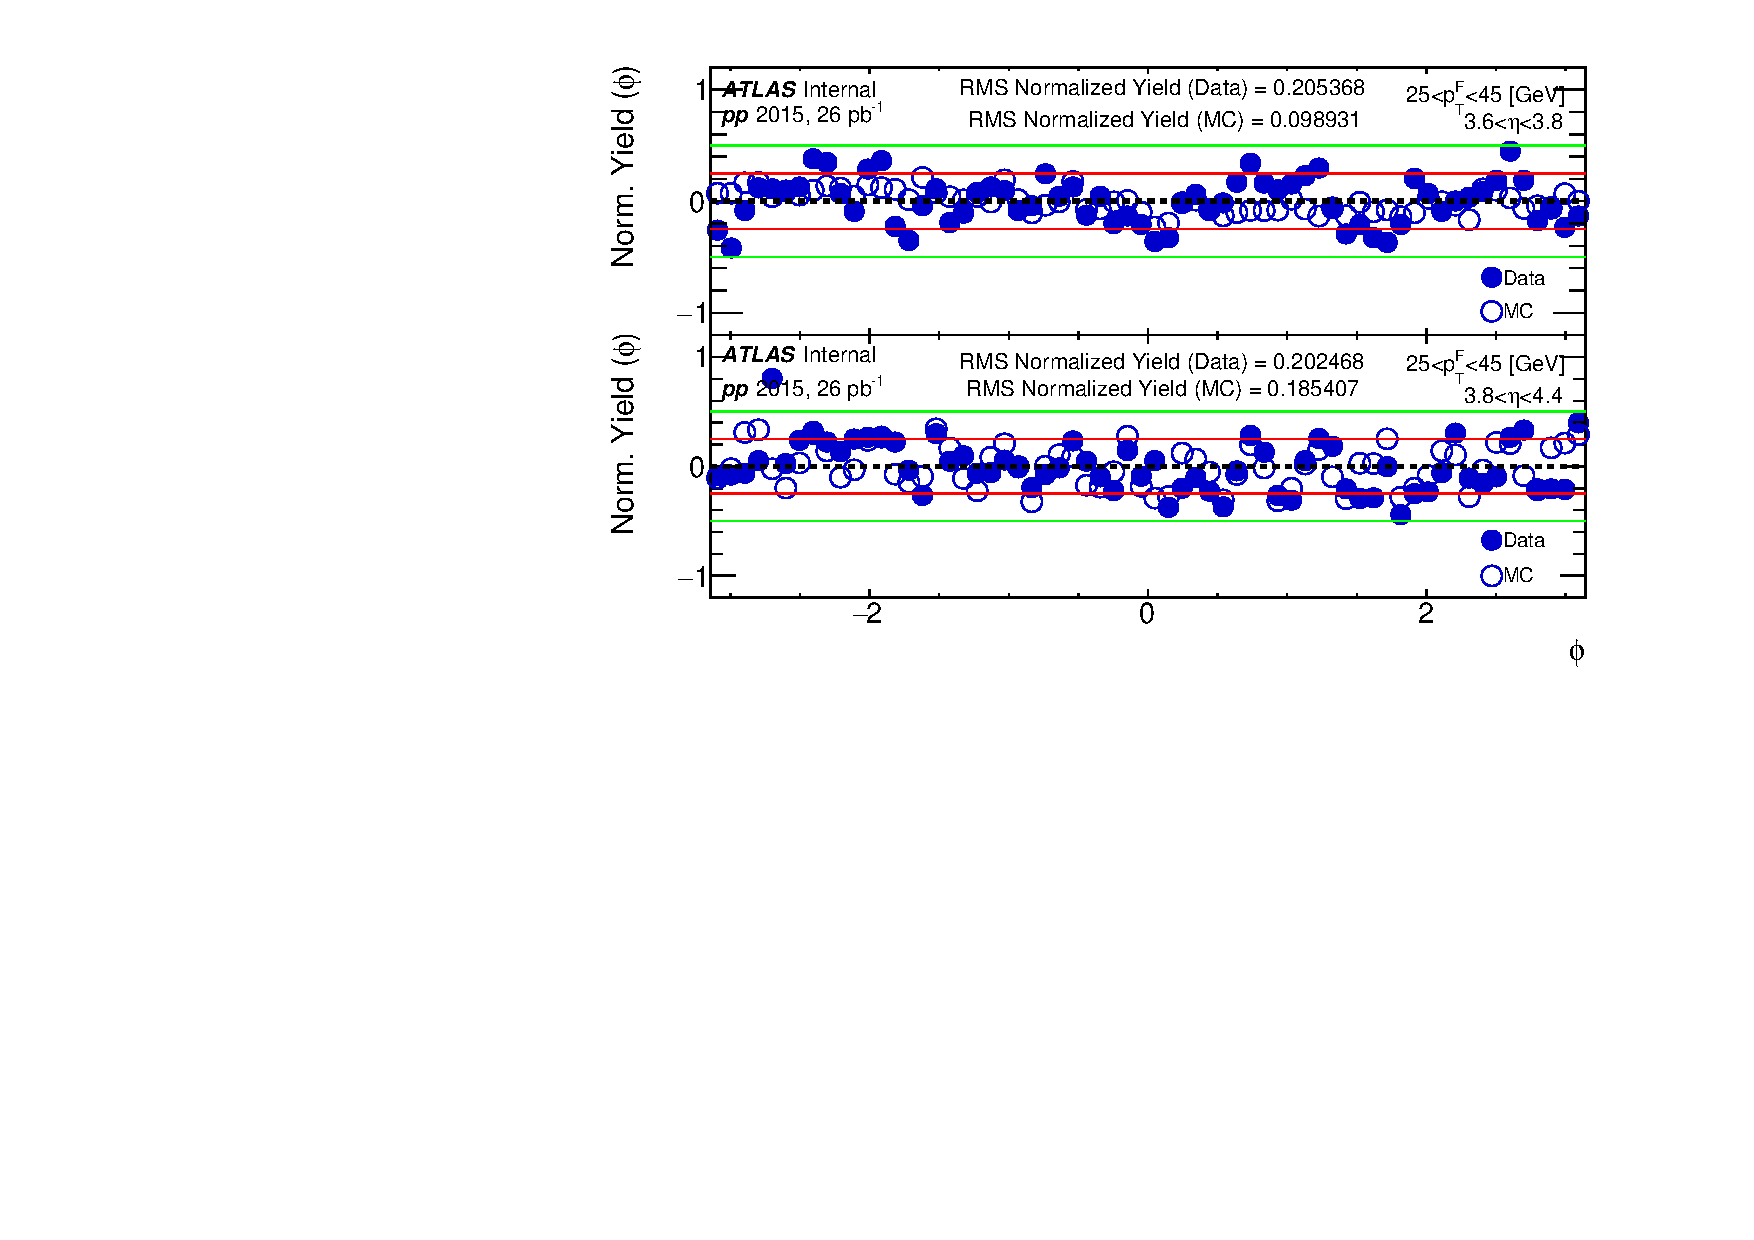
\includegraphics[width=0.8\textwidth]{figures/qualification/mcData.pdf}
	\caption{Normalized azimuthal jet yields for the forward jet $p_{T}$ bin $25<p_{T}^{Forward}<45 GeV$ is shown in the IBL region ($3.6<\eta<3.8$), and non-IBL region ($3.8<\eta<4.4$), for both data and MC. Red lines indicate a $25\%$ deviation, and green lines indicate a $50\%$ deviation.}
	\label{fig:mcdata}
\end{figure}

There is some difference seen in normalized yields between IBL and non-IBL regions. It is also important to study the $\Delta\phi$ and relative $p_{T}$ response as functions of the central jet's azimuthal angle in data and MC. The $\Delta\phi$ between forward and central jets is shown in Figure~\ref{fig:mcdatadphi}. The distribution in the data exhibits a saw-tooth pattern which is not well understood, but there does not appear to be a major difference between the IBL and non-IBL regions overall. Relative $p_{T}$ response in the forward-central dijet system is shown in Figure~\ref{fig:mcdatarpt}. Jets were required to be back-to-back, $2.5<\Delta\phi<3.8$. As with the $\Delta\phi$ distributions, no strong difference is seen between IBL and non-IBL regions. 

\begin{figure}
	\centering
	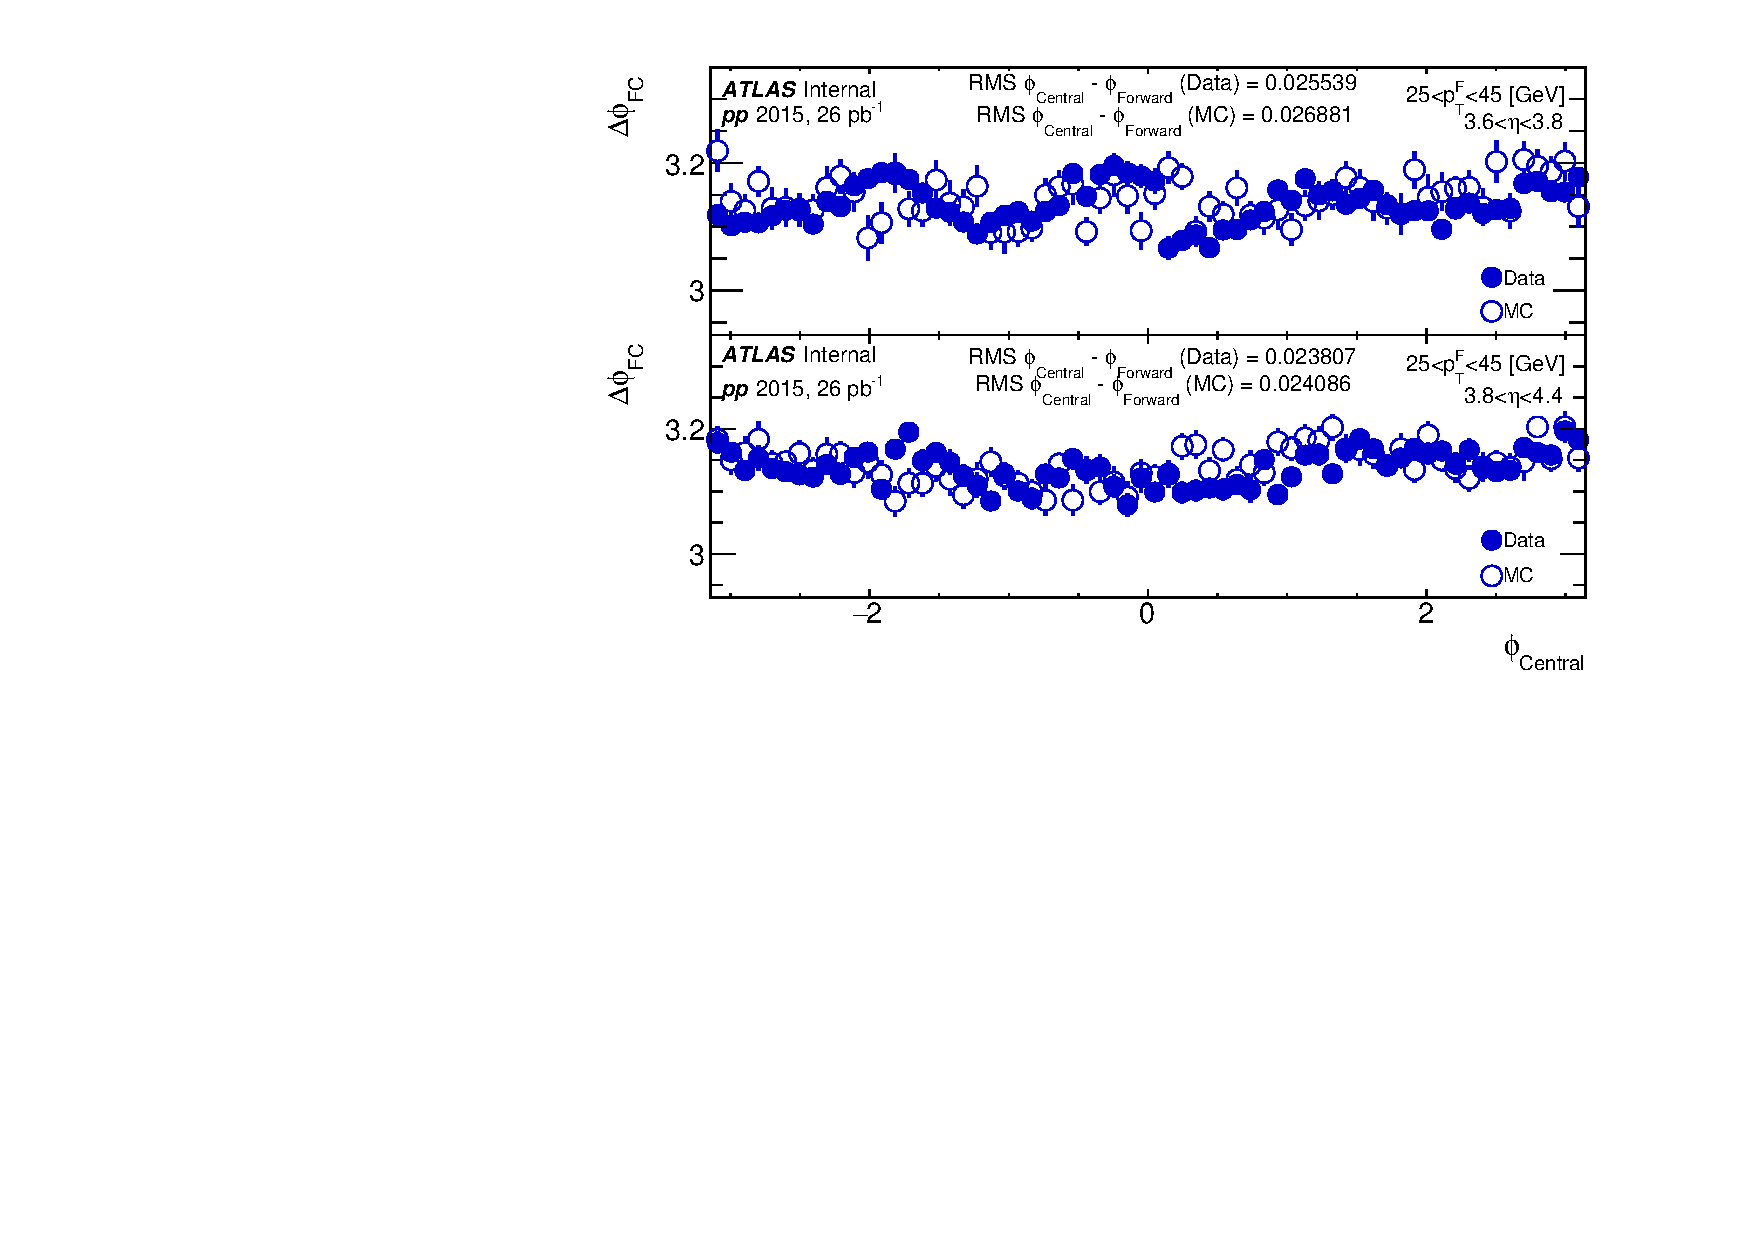
\includegraphics[width=0.8\textwidth]{figures/qualification/mcDataDPhi.pdf}
	\caption{As a function of the central jet azimuthal angle, the $\Delta\phi$ distribution for the forward jet $p_{T}$ bin $25<p_{T}^{Forward}<45 GeV$ is shown in the IBL region ($3.6<\eta<3.8$), and non-IBL region ($3.8<\eta<4.4$), for both data and MC.}
	\label{fig:mcdatadphi}
\end{figure}

\begin{figure}
	\centering
	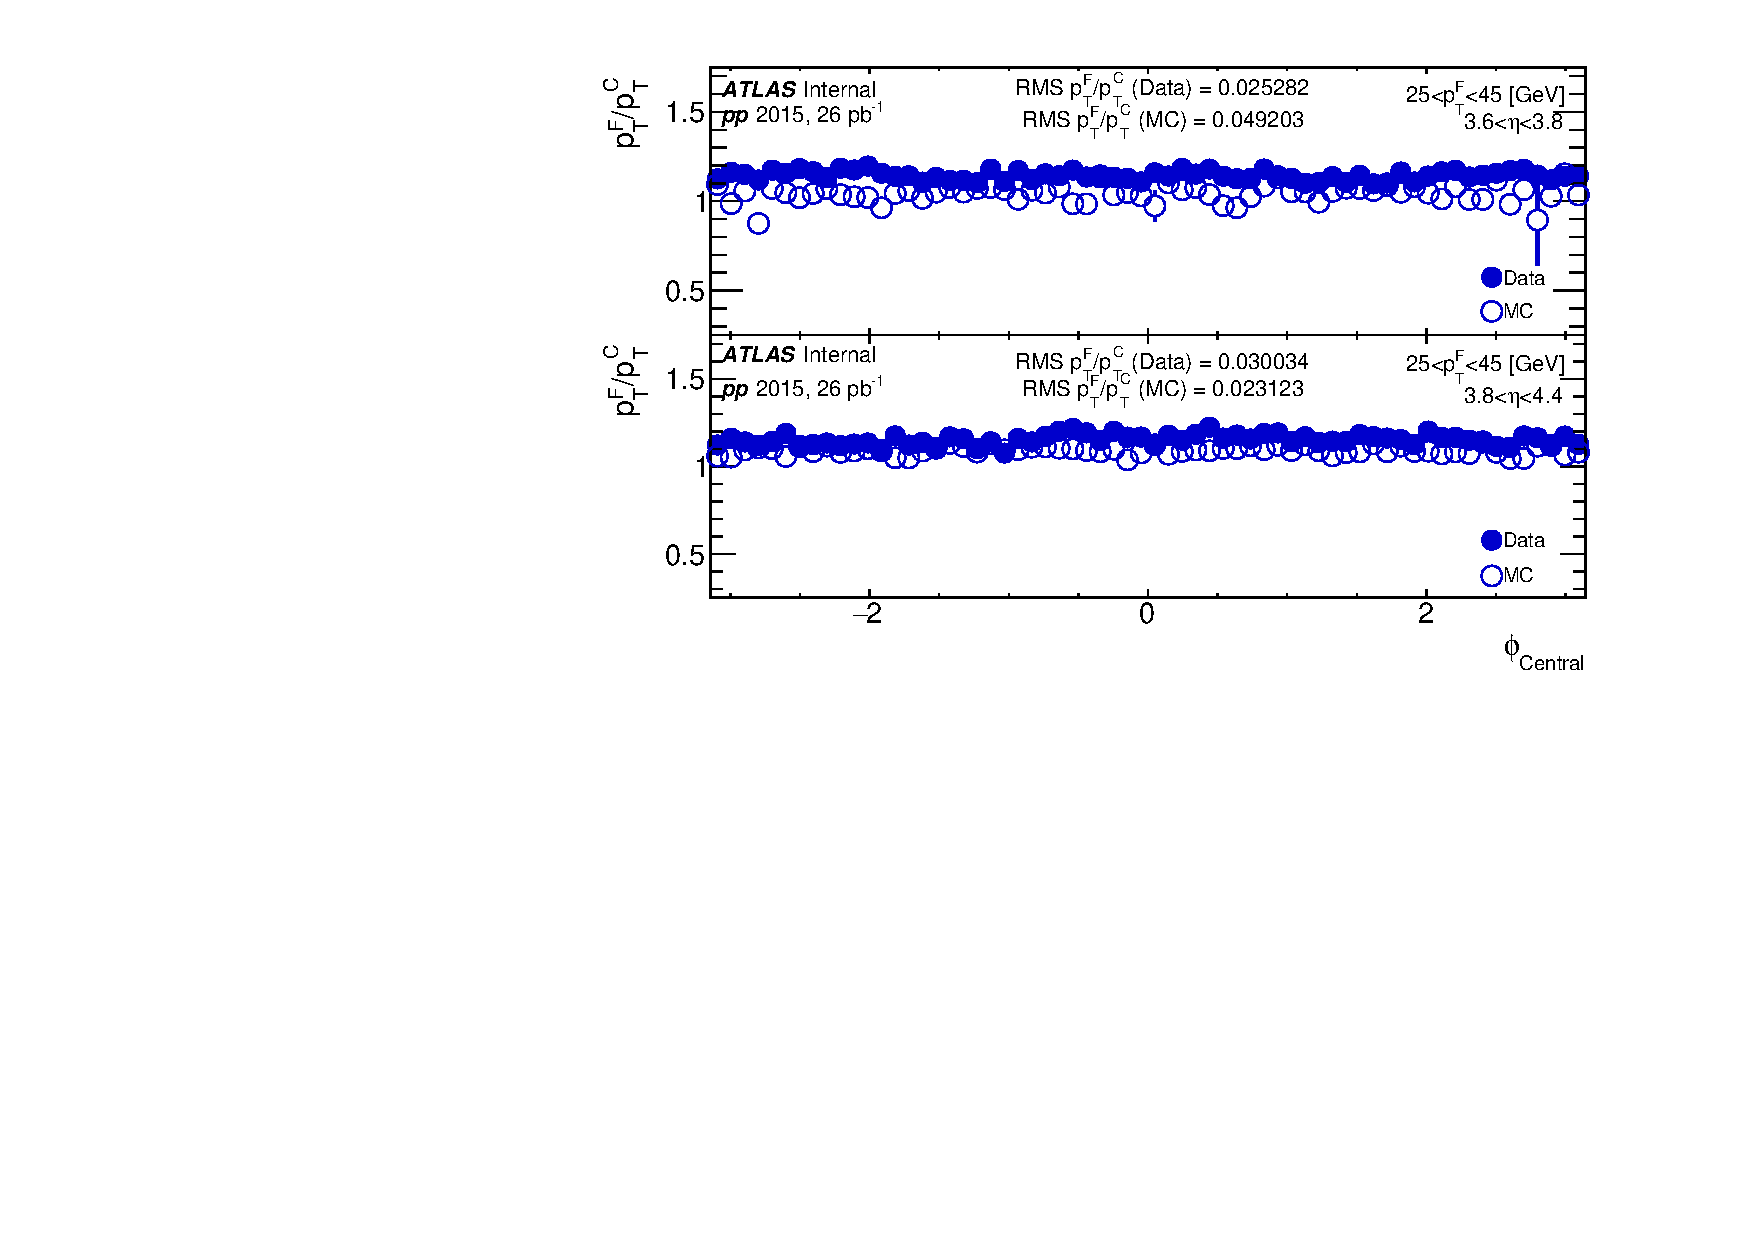
\includegraphics[width=0.8\textwidth]{figures/qualification/mcDataRPt.pdf}
	\caption{As a function of the central jet azimuthal angle, the relative $p_{T}$ distribution for the forward jet $p_{T}$ bin $25<p_{T}^{Forward}<45 GeV$ is shown in the IBL region ($3.6<\eta<3.8$), and non-IBL region ($3.8<\eta<4.4$), for both data and MC.}
	\label{fig:mcdatarpt}
\end{figure}

\section{Conclusion}

The IBL service material is found to have no significant impact on the relative $p_{T}$ response and $\Delta\phi$ azimuthal angular difference in the forward-central dijet system. This is important for the proposed thesis analysis because the forward calorimeter will be one of the most important detectors, and this study shows that the IBL material will not harm the current calibration or affect the important physical quantities. 
